\documentclass{beamer}
\usepackage{graphicx}
\usetheme{Boadilla}
\title{Area Estimation Using the Monte Carlo Method}
\subtitle{Exercise 8}
\author{Cesare De Cal}
\date{December 13, 2019}
\begin{document}

%gets rid of bottom navigation bars
\setbeamertemplate{footline}[frame number]{}

%gets rid of bottom navigation symbols
\setbeamertemplate{navigation symbols}{}

% Title page
\begin{frame}
\titlepage
\end{frame}

% Problem presentation
\section{Introduction}
\subsection{Presentation}
\begin{frame}
\frametitle{Problem Statement}
Use the Monte Carlo method to approximate the area of the figure defined by
$$
\begin{cases}
1 \le x \le 3 \\
-1\le y \le 4 \\  
x^3+y^3\le 29 \\
y \ge e^x -2
\end{cases}$$
\end{frame}

\begin{frame}
\frametitle{Bounding Box}
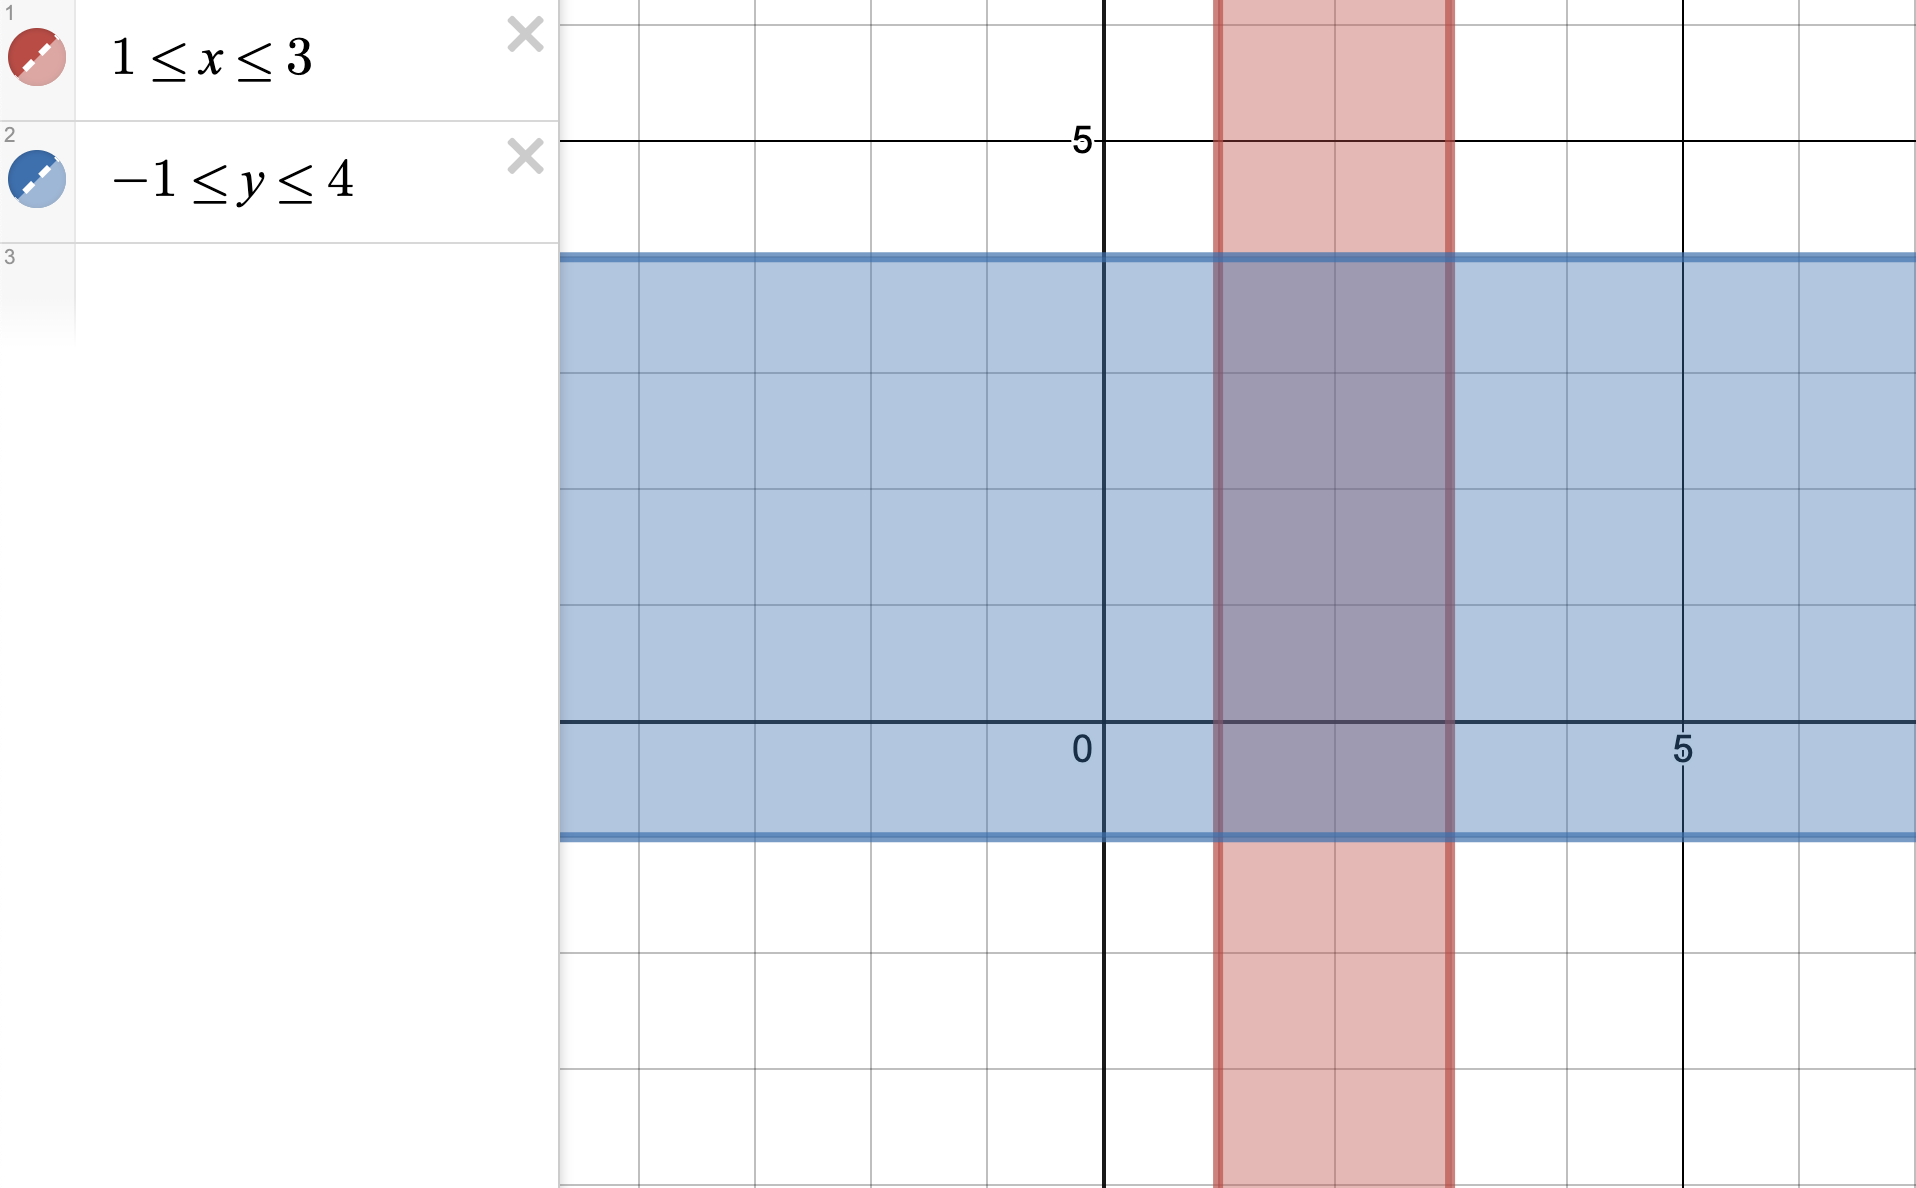
\includegraphics[width=\textwidth,height=\textheight,keepaspectratio]{bounding_box.png}
\end{frame}

\begin{frame}
\frametitle{Plot}
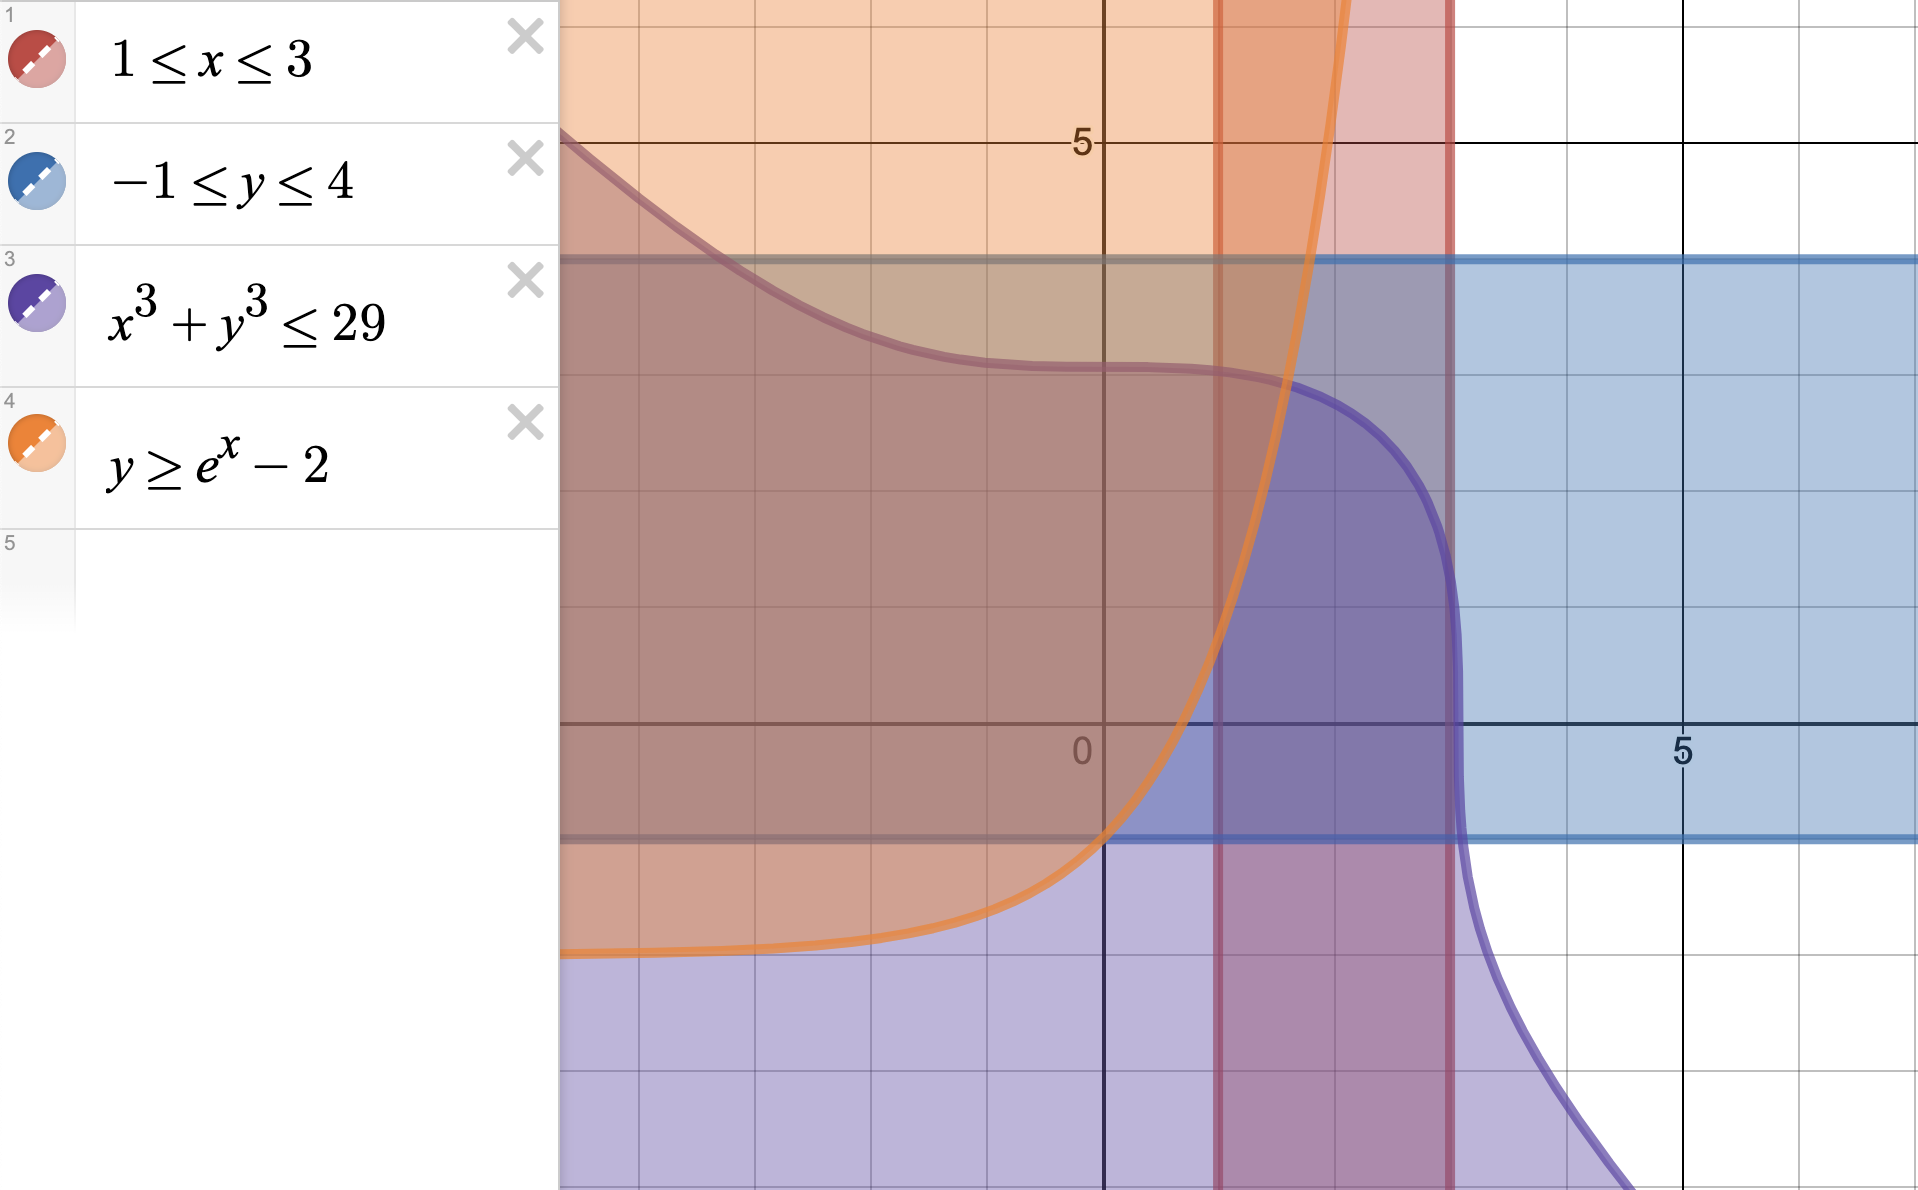
\includegraphics[width=\textwidth,height=\textheight,keepaspectratio]{full_system.png}
\end{frame}

\begin{frame}
\frametitle{Approach}
Generate N random points at random locations inside the rectangle. The area is given by:\\~\
\begin{block}{Area}
$$\textnormal{A}_\textnormal{ figure}=
\textnormal{A}_{\textnormal{ rectangle}}\times\frac{\textnormal{Points inside figure}}{\textnormal{Total points generated (N)}}$$
\end{block}
\end{frame}

\begin{frame}
\frametitle{Average of Areas}
This process is repeated LOOPS times and at the end of the N iterations the average of the areas is calculated.
\\~\
\begin{block}{Result}
For N = 30000, LOOPS = 30000, and seed equal to -87654321 the area is $7.581675111111076\times10^{-1}$.
\end{block}
\end{frame}

\begin{frame}
\frametitle{Tools}
\begin{itemize}
\item Two independent streams of random numbers with Intel MKL
\item OpenMP for multithreading
\item C Math Library for basic math functions
\end{itemize}
\end{frame}


\begin{frame}
\frametitle{Mathematical Solution}
Mathematically,
$$
\int_1^{a} (\sqrt[3]{29-x^3}-e^x+2)dx\approx 7.581218821150386\times 10^{-1}
$$
with $a=1.593743361313601$, point of intersection between the two curves defined by $y\ge e^x-2$ and $y\le \sqrt[3]{29-x^3}$.
\end{frame}

\begin{frame}
\frametitle{Observations}
Given the absolute error $4.562899606896931\times 10^{-5}$, the Monte Carlo method can be used to estimate areas with a good level of precision. Finally, OpenMP can make this computation much more efficient with multi-threading.
\end{frame}

\end{document}